\subsubsection{Dijkstra}
The Dijkstra controller lets users perform Dijkstra's Shortest Path First algorithm on a given graph.
\begin{figure}[H]
    \centering
    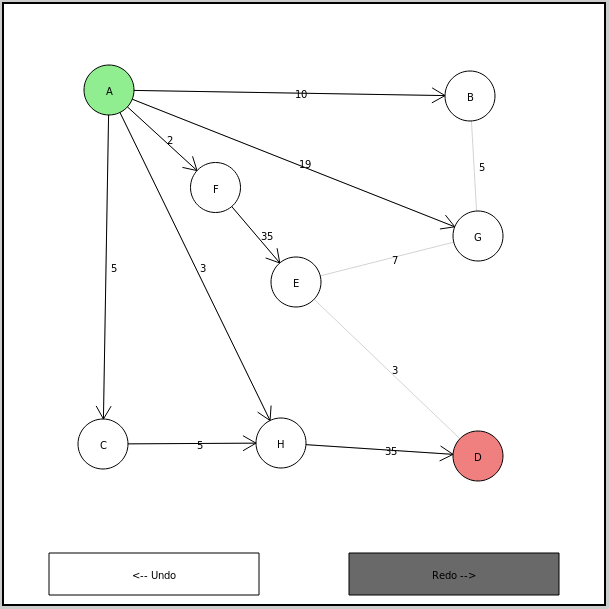
\includegraphics[width=0.7\linewidth]{/graphdrawer/dijkstraui}
    \caption{Dijkstra - user interface}
    \label{fig:graphdrawerDijkstraUserInterface}
\end{figure}
If the Dijkstra controller is not given a configuration object, then it will only display a white screen without allowing any user interaction. This happens because this controller is made for finding the shortest path, or for showing how the algorithm finds the shortest path. It can not be used to create a graph. The configuration object can determine the following properties:
\begin{enumerate}
    \item \code{steps}, should be an array of the steps the algorithm uses to find the shortest path. This can be undefined if the intention is for the student to use the algorithm to find the path. If \code{steps} is defined, then the \code{graph} configuration is not needed.
    \item \code{startColor}, the fill color used for the start node.
    \item \code{endColor}, the fill color used for the end node.
    \item \code{edgeColor}, the stroke color used for lines which show the path between nodes.
    \item \code{graph}, contains information about the graph which the student should use the algorithm on. The following list is all of the possible properties on the \code{graph} object.
    \begin{itemize}
        \item \code{graph}, contains the graph.
        \item \code{from}, should be the starting node.
        \item \code{to}, should be the end node.
        \item \code{nodes}, should be an array of node objects which the graph consists of.
    \end{itemize}
\end{enumerate}
The Dijkstra controller uses the steps array to store operations. There are three step types:
\begin{enumerate}
    \item \code{"Initial"}, is used to store information about the graph. It has the same properties as the \code{graph} configuration object.
    \item \code{"Distance"}, is used to show that the algorithm is checking the cost between to nodes. A distance step has two properties, \code{current} and \code{node} which are references to node objects. The distance step means that the algorithm is checking the cost of traveling from \code{current} to \code{node}.
    \item \code{"Path"}, is used to show the shortest path between the start and end node. The path step should only have one property, \code{path}, which is a list of the node values along the path.
\end{enumerate}
When the user is answering a Dijkstra question, their solution is stored as GraphDrawer edges. The student edges and guide (gray) lines are separated based on the \code{directed} property. The undo button works by checking if there are any directed edges in the edge array. If there is, then the student has performed an action which can be reverted. When an action is reverted, the edge is stored in the \code{redolog} array. If the \code{redolog} has entries in it, then the student can redo the action they reverted. When a new edge is created by the student, all entries in the \code{redolog} are removed. The reason for using undo/redo actions instead of letting the student remove individual edges is because when their answer is exported, their actions are based on the order of the directed edges in the GraphDrawer. If they were able to remove individual edges, the exported edges would not match what the student meant when they created them.